\documentclass[reprint,english,notitlepage]{revtex4-1}  % defines the basic parameters of the document
% if you want a single-column, remove reprint

% allows special characters (including æøå)
\usepackage[utf8]{inputenc}
\usepackage [norsk]{babel} %if you write norwegian
%\usepackage[english]{babel}  %if you write english


%% note that you may need to download some of these packages manually, it depends on your setup.
%% I recommend downloading TeXMaker, because it includes a large library of the most common packages.

\usepackage{physics,amssymb}  % mathematical symbols (physics imports amsmath)
\usepackage{graphicx}         % include graphics such as plots
\usepackage{xcolor}           % set colors
\usepackage{hyperref}         % automagic cross-referencing (this is GODLIKE)
\usepackage{tikz}             % draw figures manually
\usepackage{listings}         % display code
\usepackage{subfigure}        % imports a lot of cool and useful figure commands
\usepackage{adjustbox}

% defines the color of hyperref objects
% Blending two colors:  blue!80!black  =  80% blue and 20% black
\hypersetup{ % this is just my personal choice, feel free to change things
    colorlinks,
    linkcolor={red!50!black},
    citecolor={blue!50!black},
    urlcolor={blue!80!black}}

%% Defines the style of the programming listing
%% This is actually my personal template, go ahead and change stuff if you want
\lstset{ %
	inputpath=,
	backgroundcolor=\color{white!88!black},
	basicstyle={\ttfamily\scriptsize},
	commentstyle=\color{magenta},
	language=Python,
	morekeywords={True,False},
	tabsize=4,
	stringstyle=\color{green!55!black},
	frame=single,
	keywordstyle=\color{blue},
	showstringspaces=false,
	columns=fullflexible,
	keepspaces=true}

%% USEFUL LINKS:
%%
%%   UiO LaTeX guides:        https://www.mn.uio.no/ifi/tjenester/it/hjelp/latex/
%%   mathematics:             https://en.wikibooks.org/wiki/LaTeX/Mathematics

%%   PHYSICS !                https://mirror.hmc.edu/ctan/macros/latex/contrib/physics/physics.pdf

%%   the basics of Tikz:       https://en.wikibooks.org/wiki/LaTeX/PGF/TikZ
%%   all the colors!:          https://en.wikibooks.org/wiki/LaTeX/Colors
%%   how to draw tables:       https://en.wikibooks.org/wiki/LaTeX/Tables
%%   code listing styles:      https://en.wikibooks.org/wiki/LaTeX/Source_Code_Listings
%%   \includegraphics          https://en.wikibooks.org/wiki/LaTeX/Importing_Graphics
%%   learn more about figures  https://en.wikibooks.org/wiki/LaTeX/Floats,_Figures_and_Captions
%%   automagic bibliography:   https://en.wikibooks.org/wiki/LaTeX/Bibliography_Management  (this one is kinda difficult the first time)
%%   REVTeX Guide:             http://www.physics.csbsju.edu/370/papers/Journal_Style_Manuals/auguide4-1.pdf
%%
%%   (this document is of class "revtex4-1", the REVTeX Guide explains how the class works)


%% CREATING THE .pdf FILE USING LINUX IN THE TERMINAL
%%
%% [terminal]$ pdflatex template.tex
%%
%% Run the command twice, always.
%% If you want to use \footnote, you need to run these commands (IN THIS SPECIFIC ORDER)
%%
%% [terminal]$ pdflatex template.tex
%% [terminal]$ bibtex template
%% [terminal]$ pdflatex template.tex
%% [terminal]$ pdflatex template.tex
%%
%% Don't ask me why, I don't know.

\begin{document}



\title{Planetenes bevegelse i solsystemet}
\date{\today}
\author{Knadidatnr.: 15889}
\affiliation{Institute of Theoretical Astrophysics, University of Oslo}
\email{textme@astro.uio.no}


\newpage

\begin{abstract}
Jeg har utforsket hvordan vi kan bruke Euler-Cromer-metoden for numerisk løsning av differensiallikninger til å beregne planetbaner numerisk. Ved å ta utganspunkt i Newtons lover for gravitasjon og bevegelse har jeg funnet planetbanene i et solsystem bestående av en stjerne og syv planeter. Resultatene er sammenliknet med den analytiske løsningen vi har for dette problemet, og er funnet til å stemme godt. Dette til tross for numeriske unøyaktigheter og at jeg for enkelhets skyld har sett bort fra gravitasjonskreftene som virker fra planetene.

Jeg har så brukt samme numeriske metode for å simulere et system som består av to stjerner og én planet, denne gangen uten å se bort fra noen av kreftene. Dette problemet har ingen analytisk løsning, men ved den numeriske metoden har jeg vært i stand til å finne banene til legemene i systemet.

Deretter valgte jeg ut én av planetene i solsystemet, og gjennomførte en simulasjon av en romsondelanding på denne planeten. Landingen var suksessfull, men jeg var avhengig av å prøve og feile mye for å finne en bane som lot sonden lande uskadet. Den ble sluppet fra en satelitt i bane rundt planeten. Ved å teste mange initialverdier for hastigheten klarte jeg til slutt å simulere landingen slik at sonden hverken ble skadet av høy temperatur på vei gjennom atmosfæren eller et for hardt sammenstøt med bakken. Dette viste seg å være svært krevende for den valgte planeten.
\end{abstract}
\maketitle                                % creates the title, author, date & abstract



\section{Introduksjon}

Jeg skal beregne planetbanene i et annet solsystem numerisk. I solsystemet er det syv planeter som kretser rundt en stjerne ikke så ulik vår egen sol. Stjernen har ca. 87.9\% så stor masse og 0.4\% større radius enn solen vår. Jeg skal beregne banene ved hjelp av Newtons gravitasjonslov og Newtons 2. lov. Jeg ser bort fra kreftene som virker på stjernen og kreftene mellom planetene. Det gir oss en forenklet problemstilling som likevel gir en løsning som ikke er så langt unna virkeligheten. Problemet har en analytisk løsning som jeg kan bruke til å kontrollere resultatene fra den numeriske beregningen.

Deretter skal jeg simulere et 3-legeme-system. Vi har en planet med masse omtrent lik Mars', og to stjerner med masse på én og fire solmasser som går i baner rundt hverandre. Igjen skal jeg finne bevegelsen til legemene ved å regne ut gravitasjonskreftene som virker mellom dem, denne gangen uten å se bort fra noen av kreftene. Dette er et problem som ikke har en analytisk løsning.

Til slutt skal jeg bruke mange av de samme metodene til å simulere landing av en romsonde på en valgt planet i solsystemet jeg allerede har studert. Da må jeg i tillegg til gravitasjonskraften ta med luftmotstand i beregningene, og sørge for at denne friksjonskraften ikke blir så stor at sonden blir ødelagt. Jeg må også sørge for at farten blir lav nok før sonden treffer planeten til at den overlever sammenstøtet.

Av disse problemene er det bare det forenklede for planetbanene i solsystemet som har en analytisk løsning. Disse analytiske resultatene har begrenset anvendelighet siden vi må se bort fra kreftene som virker mellom planetene i solsystemet og fra planetene på stjerna. For å kunne gjøre beregninger på posisjonene til systemer av stjerner og planeter er vi derfor helt avhengige av å kunne bruke numeriske metoder. Det samme gjelder for problemer som er mer kompliserte fordi de inneholder andre krefter enn tyngdekraften. Dette prosjektet handler om å utforske numeriske metoder som er helt sentrale for å bedre vår forståelse av universet og dets utvikling.


\section{Teori}

Newtons gravitasjonslov sier at gravitasjonskraften på et legeme med masse $m_1$ fra et legeme med
 masse $m_2$ er
 \begin{equation}
   \label{eq:NGrav}
   \vec{F}_1 = \frac{G m_1 m_2}{r^2} \hat{\imath}_r
 \end{equation}
 der $\vec{F}_1$ er kraften som virker på legemet, $G$ er gravitasjonskonstanten, $r$ er avstanden mellom legemene og $\hat{\imath}_r$ er enhetsvektor som peker i retning fra $m_1$ mot $m_2$. Gravitasjonskraften på legeme $m_2$ er like stor men motsatt rettet: $\vec{F}_2 = -\vec{F}_1$.

Newtons 2. lov sier at akselerasjonen til et legeme er proporsjonal med nettokraften som virker på
 det:
 \begin{equation}
   \label{eq:N2}
   m \frac{\mathrm{d}^2 \vec{r}}{\mathrm{dt}^2} = \vec{F}_{\text{net}}
 \end{equation}
 Her er $m$ massen til legemet, $\vec{r}$ er posisjonen og $\vec{F}_{\text{net}}$ er nettokraften som virker på det.

Den analytiske løsningen for planetbanene når vi ser bort fra kreftene som virker mellom planetene er at de beveger seg i ellipsebaner, se figur \ref{fig:ellipse}. Utledningen av dette bygger på Newtons andre lov og gravitasjonslov, og kan finnes i \citep{part1B}. Dersom man ser bort fra kreftene som virker på stjerna, vil ellipsene ha stjerna i det ene brennpunktet ($m_1$ i figur \ref{fig:ellipse}). Vi kjenner banenes vinkling samt størrelsen på store halvakse (a i figuren) og eksentrisiteten i banene. Dermed kan vi finne avstanden mellom planetene og sola ved alle vinkler $f$ i figuren (utledningen finnes i \citep{part1B}):
 \begin{equation}
   \label{eq:analytical_ellipse}
   r = \frac{a(1 - e^2)}{1 + e \cos{f}}
 \end{equation}
 Her er $a$ lengde av store halvakse i ellipsen, $e$ er eksentrisiteten, et mål på hvor rund eller flat ellipsen er, og $f$ er vinkelen mellom posisjonsvektor fra brennpunktet i ellipsen og den rette linjen som går gjennom brennpunktet, aphel og perihel.

\begin{figure}
  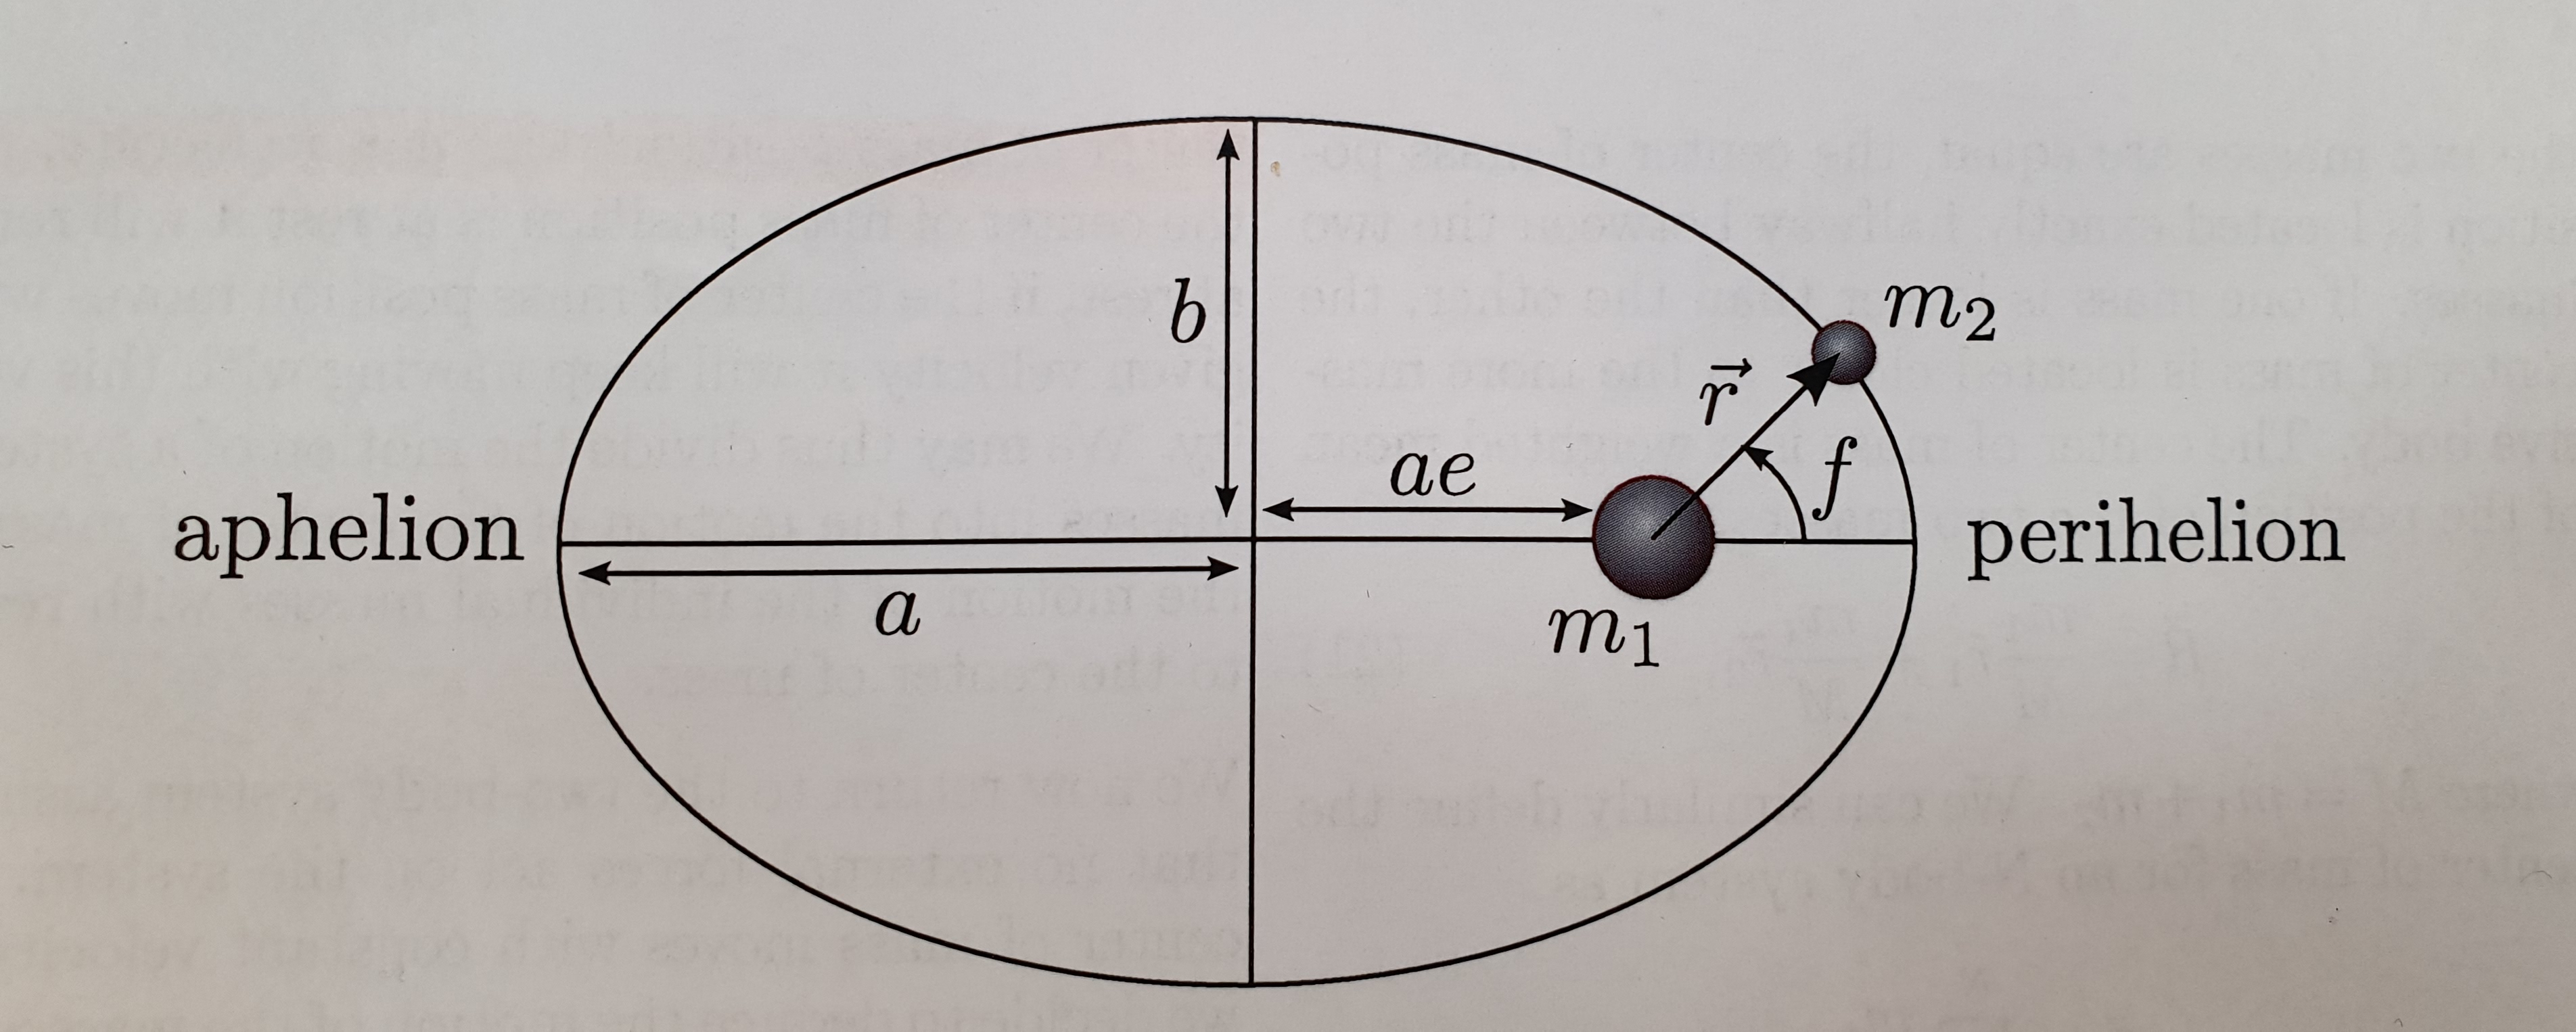
\includegraphics[width=\linewidth]{output/ellipse.jpg}
  \caption{Denne er hentet fra \citep{part1B} og viser en ellipse, den analytiske løsningen på tolegeme-problemet.}
  \label{fig:ellipse}
\end{figure}

Et legeme som beveger seg i sirkelbane med konstant banefart har total akselerasjon gitt ved uttrykket for sentripetalakselerasjon:
 \begin{equation}
   \label{eq:sentripetalakselerasjon}
   a = \frac{v^2}{r}
 \end{equation}
 der $a$ er absoluttverdien av akselerasjonen, $v$ er absoluttverdi av hastigheten og $r$ er radien i sirkelbanen. Kombinerer vi denne med Newtons 2. lov (\ref{eq:N2}) og Newtons gravitasjonslov (\ref{eq:NGrav}), får vi at banefarten til et legeme i sirkelbane er
 \begin{equation}
   \label{eq:banefart}
   v = \sqrt{ar} = \sqrt{\frac{F_{\text{net}}r}{m_1}} = \sqrt{\frac{G m_1 m_2 r}{r^2 m_1}} = \sqrt{\frac{G m_2}{r}}
 \end{equation}
 Her er $G$ gravitasjonskonstanten, $m_2$ er massen til legemet som $m_1$ går i sirkelbane rundt og $r$ er avstanden mellom massesentrene til de to legemene. Dette gjelder kun så lenge gravitasjonskraften er den eneste kraften som virker.


\section{Metode}

Vi har med likningene \ref{eq:NGrav} og \ref{eq:N2} alt vi trenger for å finne akselerasjonen til
 hver planet i ethvert punkt i banen. Jeg antar at planetene kun er påvirket av gravitasjonskraften fra stjernen og at stjernen ligger i ro, noe som gjør implementasjonen enda enklere. Ved å kombinere \ref{eq:NGrav} og \ref{eq:N2} ser vi at akselerasjonen til hver planet er gitt ved
 \begin{equation}
   \label{eq:acceleration_G}
   \frac{\mathrm{d}^2 \vec{r}_1}{\mathrm{dt}^2} = \frac{\vec{F}_1}{m_1} = \frac{G m_2}{r^2} \hat{\imath}_r = \frac{G M_{\star}}{r^3} \vec{r}
 \end{equation}
 Her er $G$ igjen gravitasjonskonstanten, $M_{\star}$ er massen til stjernen, $r$ er avstanden mellom planeten og stjernen og $\vec{r}$ er vektoren som går fra planeten til stjernen. Det betyr at akselerasjonen til planetene kun er avhengig av massen til stjernen og avstanden mellom dem. Gitt initialbetingelser for posisjon og hastighet kan vi nå beregne banene til planene ved å løse differensiallikningen
 \[\frac{\mathrm{d}^2 \vec{r}_1}{\mathrm{dt}^2} = \frac{G M_{\star}}{r^3} \vec{r}\]

For å gjøre dette bruker jeg Euler-Cromer-metoden, se \citep{part1B}. Jeg lar $\vec{r}(t)$
 være posisjonen, $\vec{v}(t)$ være hastigheten og $\vec{a}(t)$ være akselerasjonen til et legeme, alle ved et tidspunkt $t$. Initialbetingelsene er $\vec{r}(0)$ og $\vec{v}(0)$. Euler-Cromer gir da at for et lite tidssteg $\Delta t$ er
 \begin{equation}
   \label{eq:EC_vel}
   \vec{v}(t + \Delta t) = \vec{v}(t) + \vec{a}(t) \Delta t
 \end{equation}
 \begin{equation}
   \label{eq:EC_pos}
   \vec{r}(t + \Delta t) = \vec{r}(t) + \vec{v}(t + \Delta t) \Delta t
 \end{equation}
 Akselerasjonen er gitt ved likning \ref{eq:acceleration_G}. Jeg prøver meg fram for å finne et tidsintervall $\Delta t$ og et antall tidssteg som er fornuftige for at simulasjonen skal få tilfredsstillende nøyaktighet uten å ofre numerisk stabilitet. Dermed har jeg alt jeg trenger for å beregne planetenes baner rundt stjernen. Jeg skal kjøre simulasjonen til alle planetene har fullført et helt omløp. Etterpå sammenlikner jeg de numeriske resultatene med den analytiske løsningen gitt ved likning \ref{eq:analytical_ellipse}.

Perioden til planetene i sine baner kan enkelt finnes ved hjelp av Keplers tredje lov. Den sier at
\begin{equation}
  \label{eq:kepler}
  P^2 = a^3
\end{equation}
Her er $P$ perioden målt i år, og $a$ er store halvakse i ellipsen målt i astronomiske enheter.

For å simulere 3-legeme-problemet regner jeg fortsatt med at gravitasjonskraften er den eneste som virker, men denne gangen ser jeg ikke bort fra kreftene på noen av legemene. Nettokraften som virker på et legeme er summen av gravitasjoneskreftene fra de to andre. Ved å kombinere likninger \ref{eq:N2} og \ref{eq:NGrav} kan jeg igjen finne akselerasjonen til hvert legeme i enhver posisjon: \[\frac{\mathrm{d}^2 \vec{r}_i}{\mathrm{dt}^2} = \frac{\vec{F}_{i, \text{net}}}{m_i} = \sum_{j \neq i} \frac{G m_j}{r_j^3} \vec{r}_j \] Jeg løser differensiallikningen numerisk med Euler-Cromer. Jeg vil begynne simulasjonen av 3-legeme-systemet med tidssteg $\Delta t = 400$ sekunder. For små tidssteg vil kunne gi numeriske problemer og for store tidssteg gjør at resultatene blir unøyaktige.

Til slutt skal jeg simulere landingen av romsonden på den valgte planeten. Jeg antar at vi allerede har en satelitt i bane rundt planeten i en høyde 40 000km over overflaten. For å ha en myk nok landing til at fartøyet ikke blir ødelagt må hastigheten i radiell retning være mindre enn 3m/s når det treffer overflaten av planeten. Vi har en fallskjerm til hjelp, og jeg forventer å måtte prøve og feile litt for å finne en størrelse på fallskjermen som reduserer farten tilstrekkelig uten at motstanden blir for stor. Man må nemlig også passe på at friksjonskreftene (luftmotstanden) ikke på noe tidspunkt blir større enn 25 000N. Hvis friksjonskreftene blir for store vil landingsfartøyet bli revet i stykker. Jeg bruker en modell for luftmotstand som bygger på en turbulent strømning av luft rundt landingsfartøyet. Luftmotstanden er gitt ved
 \begin{equation}
   \label{eq:drag}
   \vec{F}_D = - \frac{1}{2}\rho(h)A |\vec{v}| \vec{v}
 \end{equation}
 der $\rho(h)$ er tettheten til atmosfæren som funksjon av høyden $h$ over overflaten til planeten, $A$ er arealet til fallskjermen og $\vec{v}$ er hastigheten til landingsfartøyet. Tettheten i atmosfæren i en høyde h er gitt ved
 \begin{equation}
   \label{eq:density}
   \rho(h) = \rho_0 exp(-\frac{h}{h_{\text{scale}}})
 \end{equation}
 hvor $h$ er høyden over overflaten av planeten og $h_{\text{scale}}$ er et mål på høyden til atmosfæren gitt ved
 \[
 h_{\text{scale}} = \frac{75200}{g} \text{m}
 \]
 $g$ er gravitasjonell akselerasjon ved overflaten til planeten, som er absoluttverdien av det du får ved å sette inn radien til planeten for $r$ i likning \ref{eq:acceleration_G}. $\rho_0$ er atmosfæretettheten ved overflaten av planeten. Dette er en konstant vi kjenner.

Når det gjelder størrelsen på fallskjermen er dette noe jeg kan velge selv, så lenge den ikke blir urealistisk stor. Her kan det også hende at jeg må prøve og feile for å finne en god verdi, men jeg kan også komme fram til et analytisk uttrykk for den minste størrelsen som er mulig å bruke under en suksessfull landing. Etterhvert som landingsfartøyet kommer nærmere planeten vil gravitasjonskraften gjøre at hastigheten øker inn mot sentrum av planeten. For at vi skal lande mykt må derfor luftmotstanden gjøre et stort arbeid. Luftmotstanden er proporsjonal med atmosfæretettheten, som er størst ved overflaten til planeten. Fallskjermen bør hvertfall være så stor at dersom vi har klart å senke hastigheten til 3m/s før den lander, så skal ikke farten øke igjen når fartøyet nærmer seg bakken. For at farten ikke skal øke rett før planeten treffer bakken må luftmotstanden være like stor som tyngdekraften ved $h = 0$:
 \begin{align*}
   F_G &= F_D \\
   \frac{G m M}{r^2} &= \frac{1}{2} \rho(0) A v^2 \\
   A &= \frac{2 G m M}{\rho_0 v^2 R^2}
 \end{align*}
 Her er $m$ massen til landingsfartøyet, $M$ massen til planeten, $\rho_0$ atmosfæretettheten ved overflaten av planeten, $v$ er hastigheten (3m/s) og $R$ er planetradien.

Hastigheten landingsfartøyet starter med er i utgangspunktet avhengig av banefarten til satelitten som det slippes fra, men ved hjelp rakettmotorer kan vi justere farten slik at fartøyets initialhastighet blir slik vi ønsker den. Jeg antar at banen til satelitten er sirkulær slik at farten til satelitten er gitt ved likning \ref{eq:banefart}. Jeg må velge posisjonen hvor landingsfartøyet skal bli sluppet fra satelitten, og tillegg finne en utgangsvinkel og utskytningshastighet for landingsfartøyet når det slippes fra satelitten slik at det har størst mulig sjanse for å lande trygt på planetens overflate. Her forventer jeg også å måtte prøve og feile litt.

Jeg bruker igjen Euler-Cromer-metoden for å finne posisjonen til landingsfartøyet ved alle
 tidssteg. Jeg prøver meg fram for å finne et tidssteg som gir tilstrekkelig nøyaktighet. For å sjekke at beregningene er nøyaktige nok med det valgte tidssteget, tester jeg senere med et tidssteg som er 1/10 av den valgte verdien. Programmet vil da bruke mye lenger tid på å gjennomføre beregningene. Jeg vil få et mer nøyaktig resultat, men dersom resultatet stemmer godt overens med det jeg fikk med den opprinnelige verdien av dt, kan jeg trygt bruke den opprinnelige uten å være redd for at resultatene blir veldig unøyaktige.

For å finne akselerasjonen i ett tidssteg under landingen må jeg ta hensyn til luftmotstanden i
 tillegg til gravitasjonskraften. Vi kan simpelthen legge sammen verdien for de to kreftene i \ref{eq:N2} slik at vi får
 \begin{equation}
   \label{eq:acceleration_G_D}
   \frac{\mathrm{d}^2 \vec{r}}{\mathrm{dt}^2} = \frac{\vec{F}_G + \vec{F}_D}{m}
 \end{equation}
 der $\vec{F}_G$ er gravitasjonskraften (\ref{eq:NGrav}) og $\vec{F}_D$ er luftmotstanden (\ref{eq:drag}). $m$ er massen til landingsfartøyet.




\section{Resultater}

Etter å ha implementert den numeriske og analytiske løsningen for å finne planetbanene får jeg resultatene som er illustrert i figur \ref{fig:orbits}. Likning \ref{eq:kepler} gir omløpsperioder til planetene som er listet i tabell \ref{table:periods}.
\begin{table}
\begin{adjustbox}{width=4cm}
\begin{tabular}{||c | c||}
\hline
Planet & Period, [yr]    \\ \hline
0 & 0.61    \\ \hline
1 & 1.00    \\ \hline
2 & 14.54    \\ \hline
3 & 8.72    \\ \hline
4 & 1.47    \\ \hline
5 & 22.11    \\ \hline
6 & 0.32    \\ \hline
\end{tabular}
\end{adjustbox}
\caption{Tabell som viser perioden til hver av planetene målt i år.}
\label{table:periods}
\end{table}

 \begin{figure}[htbp]
 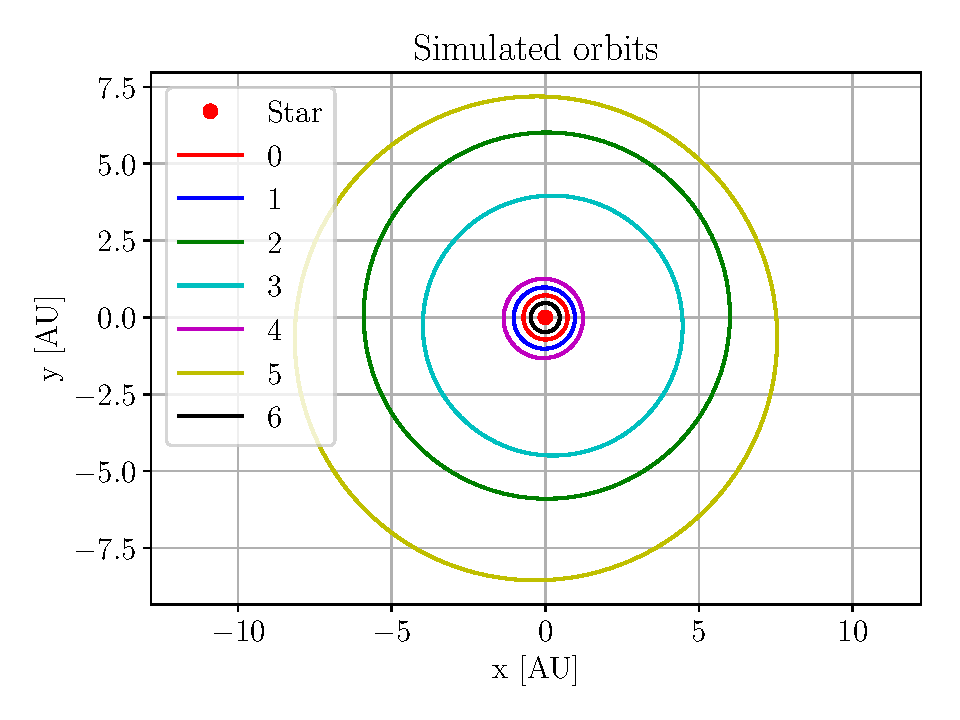
\includegraphics[width=\linewidth]{output/plots/orbits_calc.pdf}
 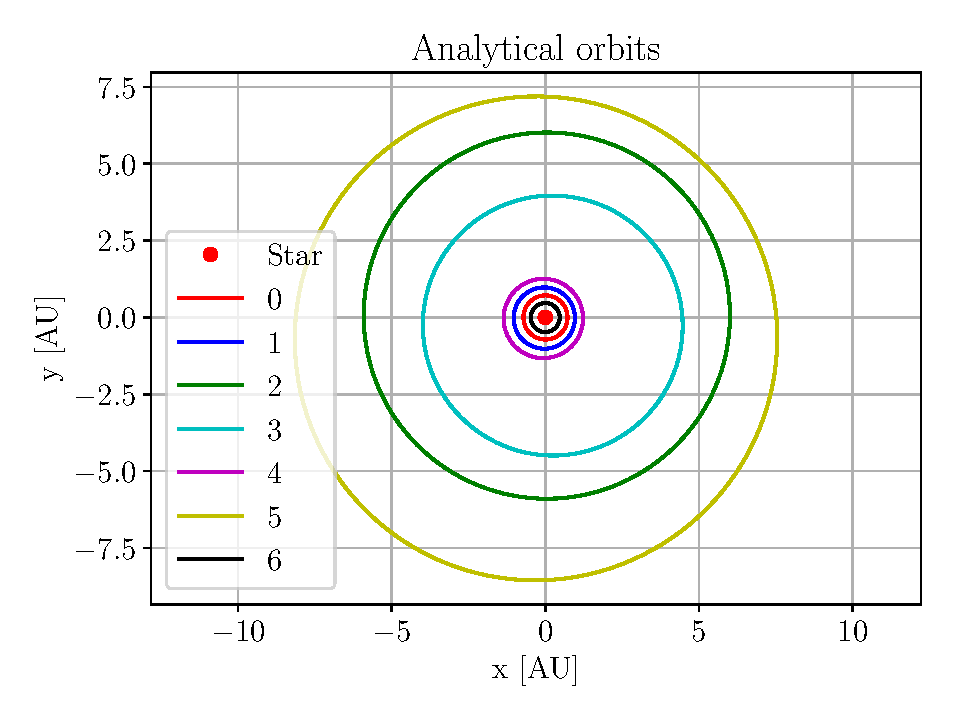
\includegraphics[width=\linewidth]{output/plots/orbits_exact.pdf}
 \caption{Banene til alle planetene i solsystemet beregnet analytisk og numerisk med $1.3 * 10^6$ tidssteg på rundt 630s. \label{fig:orbits}}
 \end{figure}

Simulasjonen av 3-legeme-systemet gir baner som er illustrert i figur \ref{fig:threebody}.
 Følgende initialbetingelser er brukt (kartesiske koordinater):
 \begin{enumerate}
   \item For planeten:
   $r_0$ = (-1.5, 0)AU,
   $v_0$ = (0, -1)km/s
   \item For stjerne 1:
   $r_0$ = (0, 0)AU,
   $v_0$ = (0, 30)km/s
   \item For stjerne 2:
   $r_0$ = (3, 0)AU,
   $v_0$ = (0, -7.5)km/s
 \end{enumerate}

 \begin{figure}
   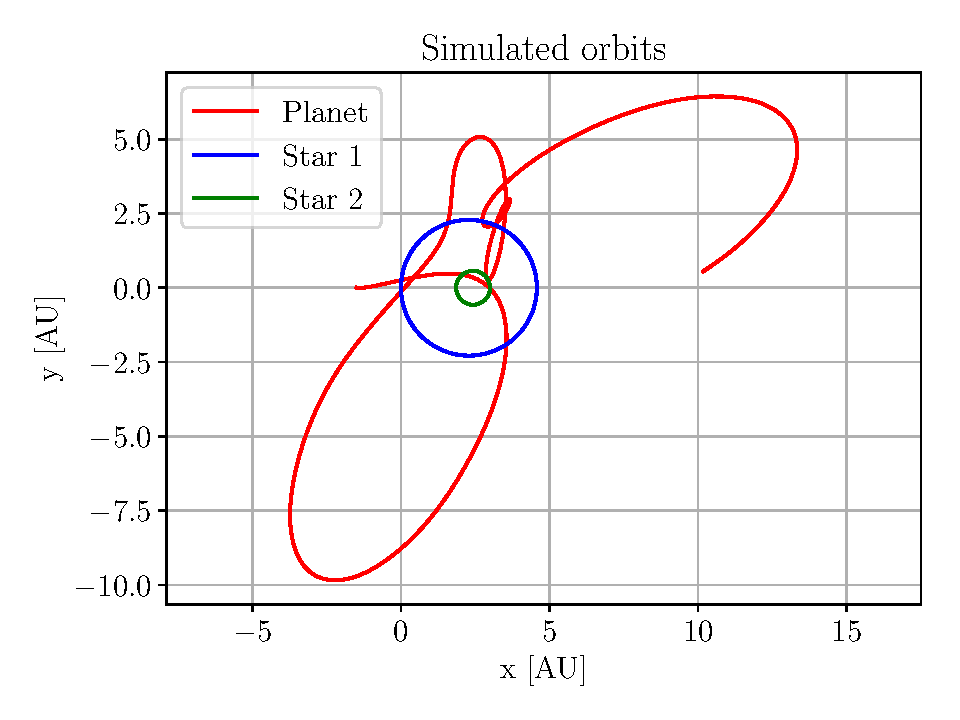
\includegraphics[width=\linewidth]{output/plots/threebody.pdf}
   \caption{3-legeme-systemet. Planeten har masse lik massen til Mars, stjerner 1 og 2 har masser på henholdsvis én og fire solmasser.}
   \label{fig:threebody}
 \end{figure}

Jeg valgte å lande på en planet med masse $1.47 * 10^{25}$kg, radius 9 692km og atmosfærisk
 tetthet $2.73 \text{kg/m}^3$ ved overflaten. Jeg brukte initialbetingelser $r_0 = (40 000 + R, 0)$km i forhold til planetens sentrum, $R$ er planetens radius, og $v_0 = (-500, 2553)$m/s. Denne verdien for hastigheten er resultatet av en del prøving og feiling. Med disse betingelsene og fallskjermstørrelse A = 100m$^2$ landet jeg på planetens overflate med radiell hastighet 2.77m/s. Tidssteget $\Delta t$ er i starten 1s, men endres til en tusendel etterhvert som landingsfartøyet kommer til tykkere atmosfære og presisjonen blir viktigere. Simulasjonen gir banen som er illustrert i figur \ref{fig:lander}.

 \begin{figure}
   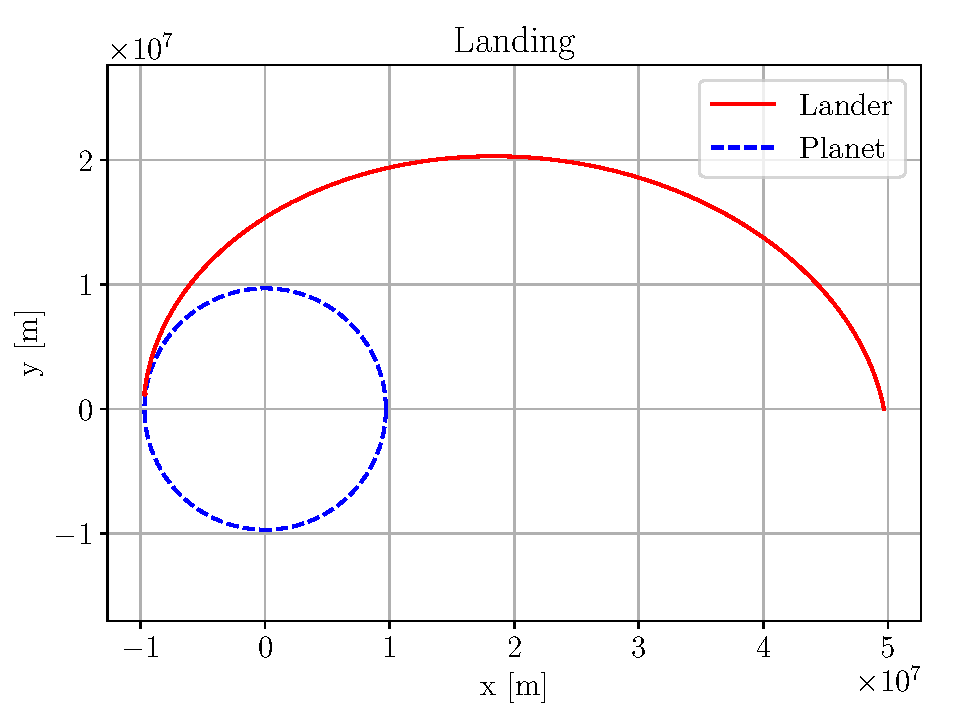
\includegraphics[width=\linewidth]{output/plots/lander_precise.pdf}
   \caption{Banen til landingsfartøyet (rødt), og planetens overflate (blått). Fartøyet lander med radiell hastighet 2.77m/s.}
   \label{fig:lander}
 \end{figure}


\section{Diskusjon}

Av likning \ref{eq:NGrav} ser vi at gravitasjonskraften som virker mellom to legemer blir større dersom massene øker. Den planeten i solsystemet som har størst masse, har bare 0.3\% så stor masse som stjernen. Det betyr at gravitasjonskreftene mellom planetene blir veldig små i forhold til kreftene som virker mellom stjernen og planetene, dette til tross for at planetene av og til er nærmere hverandre enn stjernen. Likning \ref{eq:acceleration_G} forteller også at planetene vil få mye større akselerasjon enn stjernen fordi akselerasjonen til et legeme kun er avhengig av massen til det andre legemet. I tillegg vil de forskjellige planetene, som hele tiden er fordelt rundt stjernen, trekke på stjernen i forskjellige retninger, slik at kreftene fra de forskjellige planeten kan kansellere hverandre i stor grad. Jeg antar derfor at stjernen er fast plassert i origo gjennom hele simulasjonen, og modellen vil fortsatt være en ganske god tilnærming til virkeligheten. På illustrasjonene i figur \ref{fig:orbits} ser det ut som at resultatene fra de numeriske beregningene stemmer godt med verdiene fra den analytiske løsningen. Av tabell \ref{table:periods} ser vi at omløpsperiodene er mye større for de ytre planetene enn for de innerste. Sammenliknet med vårt eget solsystem er periodene små. Mens planet 1 har samme omløpstid som jorda, er det ingen som er i nærheten av Neptuns omløpstid på 165 år.

I alle deler av dette prosjektet er jeg avhengig av å løse differensiallikninger for bevegelse. Euler-Cromer er et enkelt alternativ for å løse disse numerisk. Metoden har ikke spesielt god presisjon sammenliknet med andre metoder, og energi er ikke bevart. Energibevaring kunne blitt et problem dersom jeg skulle beregnet planetbanene for mer enn bare et par omløp, men her har det ikke spesielt mye å si. For alle eksemplene i dette prosjektet er det min vurdering at presisjonen er akseptabel så lenge man bruker et tilstrekkelig lite tidssteg. Den store fordelen med Euler-Cromer er at den er rask å implementere og rask å kjøre.

Ved å se på illustrasjonen for 3-legeme-systemet \ref{fig:threebody}, er det tydelig hvorfor dette problemet ikke har en analytisk løsning. Det ser ikke ut som at det er mulig å beskrive denne bevegelsen på samme måte som man kan beskrive ellipsebanene til planetene i tolegeme-systemet. Jeg konkluderer også med at det er lite sannsynlig at liv kan utvikle seg på denne planeten på samme måte som det har gjort på jorda. Avstanden mellom planeten og stjernene varierer voldsomt i løpet av simulasjonen. Det vil si at det er veldig store temperaturfluktuasjoner på planeten, noe som vil gjøre det vanskelig for komplekse livsformer slik vi kjenner fra jorda å utvikle seg.

Ved å bruke uttrykket for minste mulige størrelse på fallskjermen fra Teori-seksjonen får jeg at mitt landingsfartøy må ha en fallskjerm på mer enn ca. 85m$^2$. Jeg testet med noen verdier litt større enn dette, og endte opp med A = 100m$^2$.

Å finne en initialhastighet som lar meg lande mykt på planeten uten å brenne opp i atmosfæren viste seg å være krevende for denne planeten, og jeg måtte bruke ganske mye tid på å teste forskjellige verdier. Veldig lav initialhastighet gjør at fartøyet faller rett mot bakken, går raskt gjennom den tynne, øvre atmosfæren, og brenner opp etterhvert som atmosfæren blir tykkere. Initialhastigheter som ligger nær banefarten i sirkelbanen til satelitten gjør selvfølgelig at landingsfartøyet fortsetter å bevege seg i sirkelbane uten å lande på planeten.

Atmosfæren på planeten er ganske tettpakket lavt over overflaten. Det betyr at fartøyet kan falle langt mot planeten før det kommer inn i tykkere atmosfære, da med høy fart og en kort strekning igjen å bremse på. Jeg forsøkte å sende fartøyet i bane rundt planeten slik at den akkurat streifet atmosfæren ved hver passering og på den måten fikk litt og litt lavere hastighet ved hver passering, men denne metoden fikk jeg ikke til å føre fram. For å få bremset mest mulig høyt oppe i atmosfæren var det viktig å komme inn over planeten mest mulig parallelt med overflaten, for så å lande på andre siden enn den jeg startet på. Dette ser man tydelig på figur \ref{fig:lander}. Sonden må tilbringe så mye tid som mulig i de øvre lagene i atmosfæren for å få bremset mest mulig før den kommer ned i tykkere atmosfære. Det hadde vært interessant å se en illustrasjon av luftmotstanden underveis i banen for hver av de forskjellige banene jeg har testet. Siden kraften er kvadratisk proporsjonal med hastigheten til sonden, kan en liten reduksjon av hastigheten høyt oppe i atmosfæren utgjøre en stor forskjell lenger nede. Den er også proporsjonal med atmosfæretettheten, som øker eksponentielt nedover i atmosfæren. For hver $h_{\text{scale}}$ sonden beveger seg nedover mot planeten, øker tettheten med en faktor $e$. Det betyr at tettheten, og dermed også luftmotstanden vil øke svært mye i løpet av en kort avstand (kort tid og få tidssteg dersom man har høy fart) når den eksponentielle veksten begynner å gjøre seg bemerket.

Til å begynne med fikk jeg problemer med landingen fordi jeg brukte for store tidssteg. Siden atmosfæren til planeten er tett og ikke når så høyt over bakken, blir luftmotstanden raskt mye større etterhvert som fartøyet beveger seg mot overflaten av planeten. Dersom tidssteget er for stort vil tettheten øke så mye fra ett tidssteg til de neste at luftmotstanden plutselig blir for stor og gjør at fartøyet brenner opp. Ved å dele dette intervallet opp i flere mindre vil fartøyet bremse mer gradvis over flere punkter på veien. På den måten blir farten mindre når den kommer ned i tykkere atmosfære, noe som gjør at luftmotstanden blir mindre slik at sonden overlever i stedet for å brenne opp. Det er nødvendig med større presisjon lenger ned i atmosfæren, når sonden nærmer seg planeten, fordi kreftene er veldig mye større her enn langt unna. Tyngdekraften på sonden der den starter nedstigningen er bare 40N. Ved overflaten til planeten er tyngdekraften 1052N, og vi vet at luftmotstanden på vei ned nærmer seg 25 000N. Når kreftene blir så mye større, blir også akselerasjonen i hvert tidssteg mye større. Dette fører til en stor endring av bevegelsen i hvert tidssteg i forhold til størrelsesskalaen på systemet. Da er det viktig å gjøre disse beregningene ofte, så tidsstegene må være små.

For å sjekke presisjonen på løsningen etter at jeg hadde klart å lande, reduserte jeg tidssteget til en tidel og kjørte programmet på nytt. Da starter simulasjonen med $\Delta t = 0.1$s, som endres til 0.0001s etterhvert som sonden kommer ned i tykkere atmosfære. Dette ga veldig like resultater, men simulasjonen tar mye lenger tid å kjøre. Posisjonen for landingen ble stort sett den samme, og den radielle hastigheten ved landing endret seg bare med $1.2 * 10^{-7}$\%. Jeg er derfor trygg på presisjonen ved beregningene med startverdi for $\Delta t$ på 1s.



\begin{thebibliography}{}
\bibitem[Hansen (2017)]{part1B} Hansen, F. K.,  2017, Forelesningsnotat 1B i kurset AST2000


\end{thebibliography}



\end{document}
